\section{Introduction}
\label{sec:introduction}

% state the learning objective 
In this laboratory assignment we pretend to study a circuit containing two tension sources $V$, two current sources $I$ and six resistors distributed $R$ in four elementary meshes.The circuit can be seen in Figure~\ref{fig:Circuit_Base}.

In this report we start by analysing in theory the circuit (section~\ref{sec:analysis}).In Section~\ref{sec:simulation}, the circuit is analysed by
simulation, and the results are compared to the theoretical results obtained in
Section~\ref{sec:analysis}. At the end of this report we make a final conclusion to sumarise what was made along this laboratory 
(Section~\ref{sec:conclusion}).

\begin{figure}[h] \centering
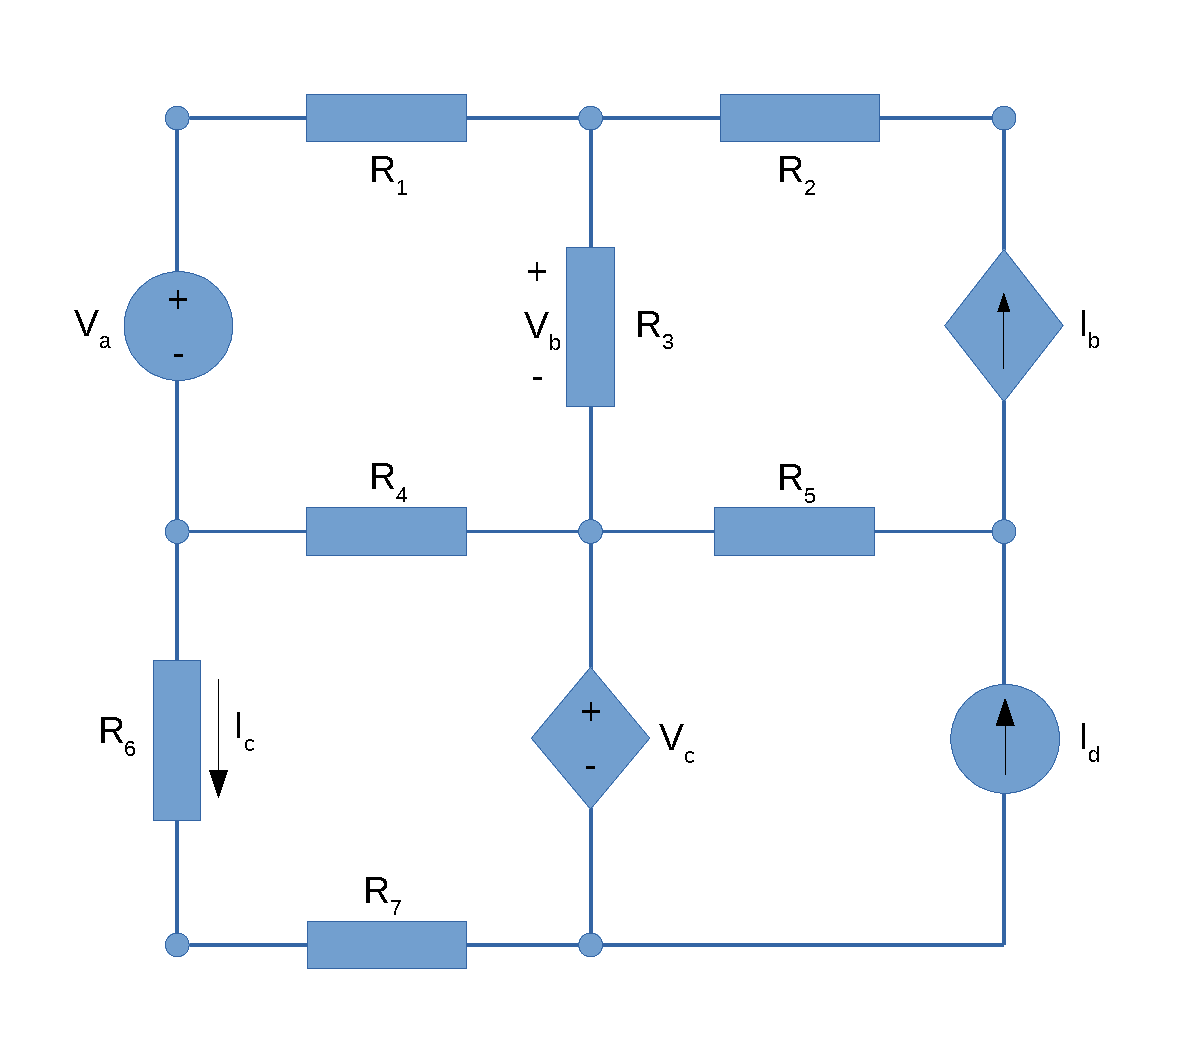
\includegraphics[width=0.5\linewidth]{Circuit.pdf}
\caption{Circuit analysed.}
\label{fig:Circuit_Base}
\end{figure}

